%\documentclass{beamer}
\documentclass[xcolor=pdftex,dvipsnames,table]{beamer}
\usepackage{verbatim}


\usetheme{Luebeck}
\usecolortheme[named=RawSienna]{structure}
\setbeamerfont{frametitle}{family=\rmfamily,shape=\itshape}
%\setbeamertemplate{frametitle}[default][center]
\defbeamertemplate*{title page}{customized}[1][]
{
  \vspace{1.9cm}

% Content  
  \begin{minipage}{10cm}
  
  % Title and subtitle
  \begin{beamercolorbox}[center,#1]{title}
    \usebeamerfont{title}\inserttitle\par%
    \ifx\insertsubtitle\@empty%
    \else%
      \vskip0.25em%
      {\usebeamerfont*{subtitle}\usebeamercolor*[fg]{subtitle}\insertsubtitle\par}%
    \fi%
  \end{beamercolorbox}%
  
  \vskip1em\par
  
  % Display author(s)
  \begin{beamercolorbox}[center,#1]{author}
    \usebeamerfont{author}\insertauthor{}
  \end{beamercolorbox}
  
  \vskip1em\par

  % Institute
  \begin{beamercolorbox}[center,#1]{institute}
    \usebeamerfont{institute}\insertinstitute{}
  \end{beamercolorbox}
  
  \vskip1em%
  
  % Date
  \begin{beamercolorbox}[center,#1]{date}
    \usebeamerfont{date}\insertdate
  \end{beamercolorbox}\vskip0.5em

  \end{minipage}
  \hspace{0.6cm}
  \vfill

  \begin{flushleft}
  {\usebeamercolor[fg]{titlegraphic}\inserttitlegraphic\par}
  \end{flushleft}
  \hfill

%  \usebeamerfont{title}\inserttitle\par
%  \usebeamerfont{subtitle}\usebeamercolor[fg]{subtitle}\insertsubtitle\par
%  \bigskip
%  \usebeamerfont{author}\insertauthor\par
%  \usebeamerfont{institute}\insertinstitute\par
%  \usebeamerfont{date}\insertdate\par
%  \usebeamercolor[fg]{titlegraphic}\inserttitlegraphic
}

\title{Deferreds}
\subtitle{Strategy for Resource Reservation in the ITVM}
\author{David Buchmann}
\institute{Cisco Systems}

\date{\today}

\begin{document}

\maketitle

\begin{frame}[allowframebreaks]{Contents}
  \tableofcontents
\end{frame}

\section{Testing}

\subsection{ITVM tests parameters}
\begin{frame}
  \frametitle{ITVM: What parameters affect reservation time?}
  \begin{itemize}
    \item Targets needed (the devices being tested) - hostname / type
    \item References needed (the devices used as references) -
      hostname / type
    \item Is matchbox - whether the test is a matchbox test
    \item Priority - default 0, the priority this test should run with
  \end{itemize}
\end{frame}

\subsection{ITVM: Test outcomes}
\begin{frame}
  \begin{columns}[cc]
  \column{1.5in}
  
\includegraphics[scale=0.33]{brian.jpg}
  \column{1.5in}
  \begin{itemize}
    \item Passed
    \item Upload failure
    \item Setup failure
    \item Killed
  \end{itemize}
  \end{columns}
\end{frame}

\section{ITVM Tasks}
\subsection{Matchbox Tests (smoke tests)}
\begin{frame}
  \frametitle{Matchbox: Y u no run faster?}
  \begin{columns}[cc]
  \column{0.7 in}
  
\includegraphics[scale=0.33]{matchbox.jpg}
  \column{2.3 in}
  \begin{itemize}
    \item The matchbox test (a.k.a our smoke test) takes a long time to start, why?
    \item Depending on product, the matchbox test
      needs different resources to run.
  \end{itemize}
  \end{columns}
\end{frame}

\section{Strategies}
\subsection{What do we want to prioritise?}
\begin{frame}
\frametitle{Prioritization}
\begin{columns}[cc]
\column{1.5in}
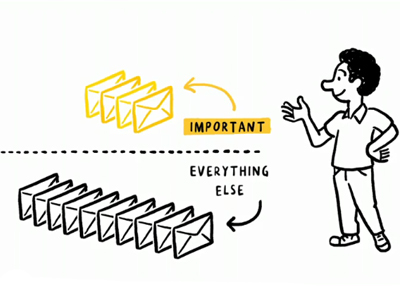
\includegraphics[scale=0.33]{priority.jpg}

\column{1.5in}
\begin{itemize}
  \item ITVMTest
  \item Matchbox
  \item Regression
\end{itemize}
\end{columns}
\end{frame}

\subsection{FIFO}

\begin{frame}
\frametitle{Naive Approach}
FIFO (first in - first out)
\begin{columns}[cc]
\column{2.0in}
\begin{itemize}
  \item Reserve sorted by oldest
  \item Stop when first test can't reserve enough
  \item Pros: simple to implement
  \item Cons: 
    \begin{itemize}
      \item lots of resources left unused
      \item matchbox tests not prioritised
    \end{itemize}
\end{itemize}
\column{0.5in}
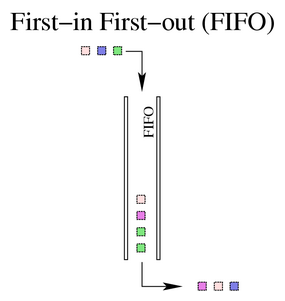
\includegraphics[scale=0.33]{fifo.png}
\end{columns}
\end{frame}

\begin{frame}
Example:
\begin{itemize}
  \item Pool has 3 snoopys and 3 falcons
  \item Task 1 requires 2 snoopies and 2 falcons
  \item Task 2 requires 1 snoopy and 2 falcons
  \item Task 3 requires 1 snoopy and 1 falcon and is a matchbox test
  \item Task 4 requires 3 snoopys
  \item Task 5 requires 1 snoopy and 1 falcon
  \item $\rightarrow$ Task 3 needs to wait for Task 1 and 2 to complete.
\end{itemize}
\end{frame}

\begin{frame}
\frametitle{Slightly less naive approach}
\begin{columns}[cc]
\column{2.0in}
Same strategy, queue sorted by
\begin{itemize}
  \item Priority (higher integer before lower)
  \item Is matchbox (true before false)
  \item Add time ascending (older before younger)
\end{itemize}
\column{0.5in}
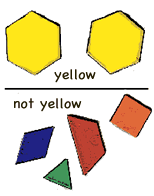
\includegraphics[scale=0.50]{sort.png}
\end{columns}
\end{frame}

\begin{frame}
Example:
\begin{itemize}
  \item Pool has 3 snoopys and 3 falcons
  \item Task 3 requires 1 snoopy and 1 falcon and is a matchbox test
  \item Task 1 requires 2 snoopies and 2 falcons
  \item Task 2 requires 1 snoopy and 2 falcons
  \item Task 4 requires 3 snoopys
  \item Task 5 requires 1 snoopy and 1 falcon
  \item $\rightarrow$ Task 3 does not wait for anyone, but when Task 4
    is running we have a lock on all snoopys so the queue will grow
    very large - we would rather run this task when the queue is small
\end{itemize}
\end{frame}

\subsection{Current Approach}

\begin{frame}
\frametitle{The current approach: First-can-first-serve}
\begin{itemize}
  \item Sorted queue from above

  \item Do \textbf{not} stop when first can not reserve
  \item Pros: Will always run the most possible tests in parallel
  \item Cons: Tests that require a lot of resources will find
    resources slower
\end{itemize}
\end{frame}

\begin{frame}
Example:
\begin{itemize}
  \item Pool has 3 snoopys and 3 falcons
  \item Task 3 requires 1 snoopy and 1 falcon and is a matchbox test
  \item Task 1 requires 2 snoopies and 2 falcons
  \item Task 2 requires 1 snoopy and 2 falcons
  \item Task 4 requires 3 snoopys
  \item Task 5 requires 1 snoopy and 1 falcon
  \item $\rightarrow$ The chance that Task 4 runs when there is a long
    queue is smaller, so we can shorten the queue and prioritise
    getting done with as many tasks as possible.
\end{itemize}
\end{frame}

\end{document}
